% version 1.00 date 08/12/2016 auteur(s) Pierre Porche
	
	Les objectifs du document, ses responsables, les documents de références ainsi que le déroulement d'une recette sont présentés dans cette partie.

\section{Objectif du document}
	Ce document présente le \PTV{} du logiciel produit par l'équipe \nomEquipe{}.
	
\section{Responsabilité}
	Les responsables de ce document sont le \CP, le \RQ{} et le \RD.
	
\section{Document de référence}
	Le \PTV{} fait référence au \DSE.
	
\section{Déroulement d'une recette}
Le déroulement d'une recette est expliqué dans ce paragraphe et par la figure \ref{deroulementDUneRecetteImage} \\

Un premier cahier de recette vierge est envoyé pour une approbation des tests de validation.
\begin{itemize}
	\item Soit le cahier de recette est approuvé;
	\item Soit le cahier de recette n'est pas approuvé, il est alors corrigé puis de nouveau envoyé pour approbation.
\end{itemize}
Ensuite se déroule la recette provisoire où sont envoyés le cahier de recette et le lot.
\begin{itemize}
	\item Soit aucune remarque n'est remontée sur le lot, il est donc approuvé par le client. Le cahier de recettes provisoire devient définitif et il y a diffusion finale du lot. 
	\item Soit des remarques sont remontées lors de la recette, le lot n'est pas approuvé, le lot passe donc en période probatoire.
\end{itemize}
Durant la période probatoire, le lot est corrigé en fonctions des remarques exprimées par le client dans le cahier de recette provisoire. La période probatoire dure minimum 3 jours et au maximum une semaine. \\
Enfin se déroule la recette définitive où sont envoyés le cahier de recette définitif et le lot corrigé. De même que précédemment plusieurs scénarii sont possibles :
\begin{itemize}
	\item Aucune remarque sur le lot, le lot est approuvé, il y a donc diffusion finale du lot;
	\item Des remarques mineures sont soulevées sur le lot, le lot est donc corrigé en conséquence, vient ensuite une approbation définitive du lot avant la diffusion finale du lot;
	\item Le lot est accepté avec report de fonctionnalités;
	\item Des remarques majeures sont soulevées sur le lot, il n'est donc pas approuvé. Il y a alors retour en période probatoire.
\end{itemize}

\begin{figure}[H]
	\centering
	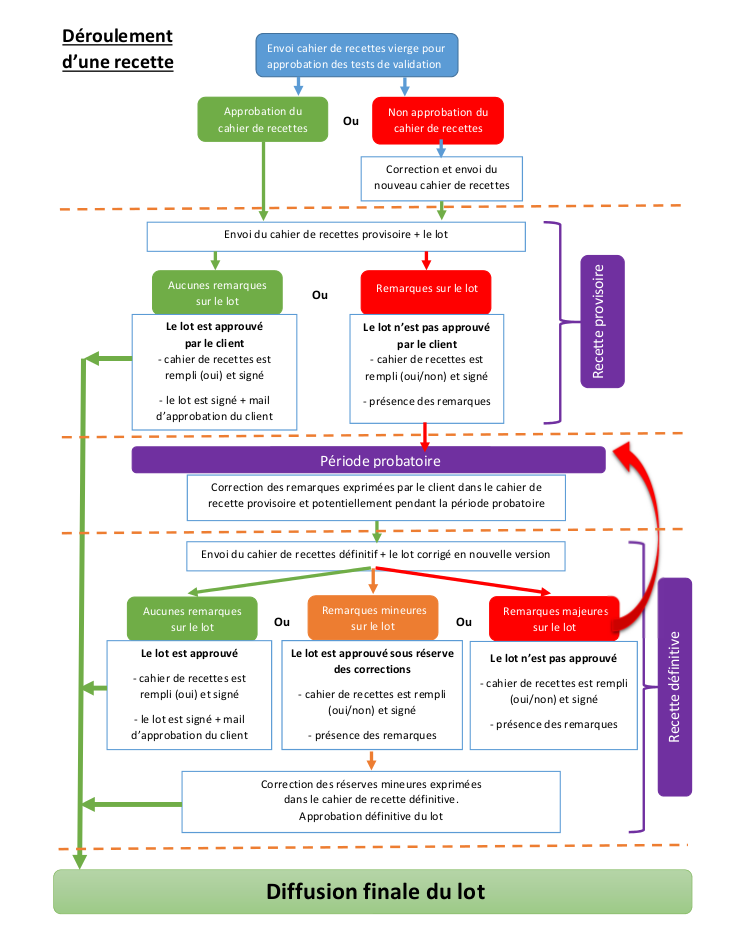
\includegraphics[scale=0.72]{images/deroulementDUneRecette.png}
	\caption{Déroulement d'une recette}
	\label{deroulementDUneRecetteImage}
\end{figure}

